\documentclass{book} \usepackage[utf8]{inputenc} \usepackage[brazil]{babel}
\usepackage{graphicx} \usepackage{amssymb} \usepackage{multicol}

\title{Livro de receitas} \author{Karl Jan Clinckspoor} \date{\today}

% Comandos customizados
\newcommand{\receita}[3]{
  \section{#1}
  \textbf{Ingredientes} #2
  \noindent \textbf{Preparo} #3
  \clearpage
}
%%%%%%%%%%%%%%%%%%%%%%%%%%%%%%%%%%%%% 
\newcommand{\fotoreceita}[2]{
  \begin{center}
    \includegraphics[width=#1]{#2}
  \end{center}
}
%%%%%%%%%%%%%%%%%%%%%%%%%%%%%%%%%%%%% 
\newcommand{\grau}{$^\circ$}
%%%%%%%%%%%%%%%%%%%%%%%%%%%%%%%%%%%%% 
\begin{document}

\maketitle
\tableofcontents

\chapter{Receitas salgadas}
\begin{center}
	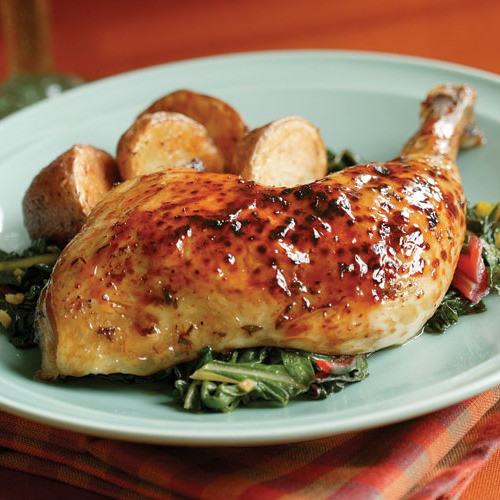
\includegraphics[width=0.7\textwidth]{Fotos/foto_savory}\end{center}
\clearpage
\receita{Stir Fry de Frango\checkmark}{
	\begin{itemize}
		\item 1 meio-peito de frango
		\item Verduras apropriadas (cenoura, brócolis, acelga)
		\item 1 dente de alho
		\item Molho shoyu
		\item Óleo para fritar
		\item Gengibre, bem pouco.
	\end{itemize} }{
	\begin{enumerate}
		\item Cortar o frango em tirinhas
		\item Ralar 1 dente de alho inteiro.
		\item Colocar um pouco de óleo numa frigideira ou wok, e colocar o alho ralado
		      e gengibre por alguns segundos.
		\item Colocar o frango quando a panela já estiver quente. Virar bastante para
		      não deixar queimar.
		      \begin{itemize}
			      \item Se não estiver quente o suficiente, o frango irá perder água e vai
			            ficar seco.
			      \item Se tiver muito frango, fazer a fritura do mesmo em várias porções, de
			            acordo com o tamanho da frigideira e da potência do fogo.
		      \end{itemize}
		\item Quando dourado, retirar o frango e colocar armazenado em outro lugar.
		\item Fritar as verduras e legumes até ficarem cozidas.
		      \begin{itemize}
			      \item Colocar sempre os mais duros antes
			      \item Caso tenha brócolis, branquear (ferver água, deixar 2-3 minutos,
			            escorrer)
			      \item Caso tenha acelga, coloque por último
		      \end{itemize}
		\item Voltar o frango, aquecer um pouco, colocar 1 colher de sopa de shoyu,
		      mexer bem para incorporar. Vai ficar mais escuro do que aparenta no
		      início. \begin{itemize} \item Se tiver macarrão, colocar o shoyu antes,
			            incorporar, depois colocar o macarrão. \item Tomar cuidado com não deixar
			            a tampa do shoyu sair e derramar demais. \end{itemize}
	\end{enumerate}

	\fotoreceita{0.7\textwidth}{./Fotos/Stir_Fry.png} }

\receita{Bife com Curry\checkmark}{
	\begin{itemize}
		\item Carne
		\item Alho
		\item Cebola
		\item Óleo/manteiga
		\item Curry em pó
	\end{itemize} }{
	\begin{enumerate}
		\item Cortar a carne em tiras
		\item Fritar cebola e alho bem picadinho, refogar com óleo ou manteiga,
		      colocar a carne e refogar uns minutos.
		      \begin{enumerate}
			      \item Como vai usar curry, pode soltar água da carne.
			      \item Caso não solte a água, abaixa o fogo e coloca a tampa e espera um
			            pouco. Caso não solte ainda, coloca meio copo de água quente.
		      \end{enumerate}

		\item Aí põe algo como uma colher de sopa de curry e termina de refogar. Serve
		      com arroz.
	\end{enumerate} }

\receita{Arroz padrão na panela de arroz\checkmark}{
	\begin{itemize}
		\item Arroz normal. Geralmente, para 2, um copo é o suficiente.
		\item Alho. Para 2, meio alho está bom.
		\item Cebola. Para 2, meia cebola pequena está bom
		\item Óleo. Suficiente para cobrir o fundo da panela com um filmezinho.
		\item Água quente
	\end{itemize}
}
{
	\begin{enumerate}
		\item (Opcional) Colocar a água para esquentar. Se fizer isso, diminui o
		      tempo de cozimento.
		\item Colocar o alho e cebola finamente picados numa panela com óleo para
		      dourar.
		      \begin{itemize}
			      \item Pode adicionar o alho depois para diminuir a
			            chance de queimar ele.
		      \end{itemize}
		\item Colocar o arroz e fritar um pouquinho. Transferir tudo para a panela de
		      arroz. Colocar a água na proporção de 2 copos de água para 1 copo de arroz
		      (medida da panela).
		\item O tempo médio de cozimento registrado aqui é de aproximadamente 13-15
		      minutos.
		\item O fundo da panela sempre fica grudado. Tentar achar uma maneira de
		      fazer isso parar de acontecer.
	\end{enumerate}
}

\receita{Arroz arbório na panela de arroz\checkmark}{\label{rec:arroz_arborio_panela}
	\begin{itemize}
		\item Arroz arbório, ou algum tipo de arroz para risoto
		\item Água, na proporção aproximada de 2x o ``volume'' de arroz.
	\end{itemize}
}{
	\begin{enumerate}
		\item Colocar o arroz arbório na panela e colocar a água. Deixar cozinhar.
		\item O resultado é um arroz que parece arroz japonês. Fica bem fofinho,
		      expandido, e contrasta bem com pratos mais fortes, como frango tailandês ou
		      outros \emph{stir-frys}.
	\end{enumerate}
}

\receita{Pique Macho\checkmark}{
	\begin{itemize}
		\item Batata para fritar
		\item Cebola roxa
		\item Tomate
		\item Pimentão (locoto)
		\item Salsicha
		\item Lombo
		\item Pimenta do reino
		\item Cominho
		\item Mostarda
		\item Shoyu (relativamente pouco, 2 colheres para 1kg de carne)
		\item Sal
		\item Óleo de girassol
		\item Ovos
		\item Maionese
		\item Ketchup
	\end{itemize} }{
	\begin{enumerate}
		\item Fritar as batatas
		\item Fritar a carne, sem se preocupar em selar. Parte do sabor do prato vem
		      do líquido soltado pela carne.
		\item Colocar o cominho, pimenta, mostarda, shoyu e sal com a carne ainda
		      vermelha.
		\item Colocar os ovos para cozinhar em outra panela.
		\item Deixar a carne cozinhar.
		\item Colocar a salsicha e esperar 5 minutos, desligar o fogo.
		\item Colocar a carne sobre as batatas fritas.
		\item Colocar as cebolas que estavam no vinagre para perder o sabor forte,
		      tomate, ovos cozidos, pimentões verdes, sobre o prato.
	\end{enumerate}

	\fotoreceita{0.7\textwidth}{./Fotos/pique_macho}

}

\receita{Macarrão com manteiga, ovo e queijo\checkmark}{
	\begin{itemize}
		\item Espaguete (80 g para uma pessoa)
		\item Sal
		\item 3/4 copo de leite
		\item 1 ovo
		\item 2 colheres de manteiga
		\item 2/3 copo de parmesão ralado
		\item Pimenta a gosto
	\end{itemize} }{
	\begin{enumerate}
		\item Cozinhar o macarrão numa panela. \begin{itemize}
			      \item Colocar sal na água. Deixar ferver. Colocar macarrão.
		      \end{itemize}
		\item Escorrer o macarrão ao ficar al dente.
		\item Devolver o macarrão na panela, abaixar a temperatura, colocar a mistura
		      de leite, ovo e manteiga, e mexer até recobrir o macarrão. \begin{itemize}
			      \item Quando eu fiz, deixei bastante tempo para garantir que o ovo estivesse
			            cozido. Ele engrumou, mas a Karen gostou de qualquer forma.
		      \end{itemize}
		\item Remover o calor. Colocar queijo e misturar. Se estiver pastoso demais,
		      colocar mais lente.
	\end{enumerate} }

\receita{Caldo de frango\checkmark\label{rec:caldo_frango}}{
	\begin{itemize}
		\item 3 dentes de alho
		\item 1 cebola pequena
		\item 2 coxas de frango, 2 sobrecoxas de frango, 2 meio-peitos
		\item Óleo
		\item Sal
	\end{itemize} }{
	\begin{enumerate}
		\item Cortar bem pequeno o alho e a cebola. Colocar ambos para dourar um pouco
		      de tempo. Colocar uma colher de chá de sal.
		\item Colocar o frango, sem tirar a pele ou qualquer outra coisa.
		\item Colocar a água. Cerca de 2 litros, ou até cobrir tudo. Deixar a panela
		      no fogo alto até a água começar a ferver, depois colocar no fogo médio.
		\item Tempo total é de cerca de 1h depois de começar a ferver. Mexer no frango
		      de vez em quando para ver a textura e possivelmente abrir os pedaços para
		      ajudar a cozinhar.
		      \begin{itemize}
			      \item Dá para remover o peito antes dos outros porque deve cozinhar antes, e
			            se ficar tempo demais fica duro.
		      \end{itemize}
		\item Estará pronto quando notar que a carne está saindo dos ossos.
		\item Coar tudo por uma peneira. Reservar o frango para fazer uma torta ou
		      alguma coisa assim.
	\end{enumerate} }

\receita{Risoto de parmesão\checkmark}{
	\begin{itemize}
		\item 2,5 copos de caldo de frango (vide receita \ref{rec:caldo_frango})
		\item 0,75 copos de água
		\item 2 colheres de sopa de manteiga
		\item 0,5 cebola grande, finamente cortada
		\item Sal, pimenta
		\item 0,5 dente de alho, cortado finamente
		\item 1 copo de arroz para risoto (arbório ou outro)
		\item 25-30g de parmesão ralado
		\item 1 colher de sopa de salsinha e cebolinha
		\item 0,5 colher de sopa de suco de limão
	\end{itemize} }{
	\begin{enumerate}
		\item Ferver o caldo e a água em panela grande em fogo quente. Depois reduzir
		      o calor para um fervor gentil.
		\item Derreter metade da manteiga numa panela\footnote{De preferência de
			      ferro, mas pode ser alguma com uma massa térmica maior que uma panela
			      comum} em calor médio. Colocar a cebola e 0,75 colher de sopa de sal. Ir
		      mexendo por 5 a 7 minutos.
		\item Colocar o alho até ficar cheiroso, 30 segundos.
		\item Colocar o arroz e cozinhar, mexendo lentamente até os grãos ficarem
		      translúcidos nas bordas, 3 minutos.
		      \begin{itemize}
			      \item Cuidado com deixar o arroz queimar nesta etapa! Mexer bastante.
		      \end{itemize}
		\item Colocar o caldo aquecido até cobrir o arroz. Reduzir o calor para
		      médio-baixo. Ficar mexendo até absorver. Quando secar, adicionar mais caldo
		      em parcelas bem pequenas. Sempre ficar mexendo para garantir que não vai
		      queimar. Continuar até o arroz ficar cremoso e cozido, ou acabar o caldo.
		      16-19 minutos.
		\item Colocar o parmesão e mexer. Remover do calor, cobrir, e deixar parado
		      por 5 minutos.
		\item Colocar o resto da manteiga, salsinha, cebolinha e limão.
		      \begin{itemize}
			      \item O limão não foi muito bem quisto pela Karen. Dá para colocar a
			            salsinha e cebolinha, separar em duas metades, e em uma delas colocar 0,25
			            colher de sopa do suco de limão.
		      \end{itemize}
	\end{enumerate}

	\fotoreceita{0.7\textwidth}{./Fotos/Risoto.png} }

\receita{Conchiglioni de queijo\checkmark}{
	\begin{itemize}
		\item Aproximadamente 50 Conchiglioni
		\item 1 cilindro de ricota fresca. Mais molinha é melhor (cerca de 200g?)
		\item 1 pote de creme de ricota.
		\item 100g de mussarella ralada
		\item 100g de provolone ralado
		\item 25g de parmesão ralado para recheio, um pouco para polvilhar em cima
		\item molho de tomate pronto. 1 saquinho para pouco molho, 2 para banhar bem.
		\item sal
		\item nozes picadas, aproximadamente 8
	\end{itemize} }{
	\begin{enumerate}
		\item Cozinhar os conchiglioni em água com sal até ficarem no ponto.
		\item Enquanto cozinha, misturar todos os queijos juntos, com as nozes. Provar
		      se tem sal suficiente e colocar um queijo ou outro para atingir o sabor.
		      Senão, colocar sal, mas por experiência, para meu gosto, isso não é
		      necessário.
		\item Ao terminar, coar o macarrão, deixar esfriar um pouco. Começar a aquecer
		      o forno a 200 $^\circ$C.
		\item Numa travessa grande, cobrir a base com molho de tomate, para evitar do
		      macarrão queimar durante o assamento.
		\item Preencher generosamente os conchiglioni com o recheio. Colocar na
		      travessa da maneira mais eficiente possível, porque 50 conchiglioni é
		      bastante.
		\item Jogar molho por cima deles, tentando ser homogêneo, mas não é
		      necessário. Após, salpicar parmesão a gosto.
		\item Colocar no forno por 15 minutos. Se tiver duas travessas, retirar a
		      travessa de baixo, mais perto do fogo, antes, para que não queime. O
		      interessante é derreter o recheio e aquecer tudo, pois a comida já está
		      tecnicamente pronta para ser comida.
		\item Servir e comer imediatamente. O que sobrar pode ser resfriado ou
		      congelado e posteriormente aquecido no micro ondas que não há perda de
		      sabor.
	\end{enumerate}

	\fotoreceita{0.5\textwidth}{./Fotos/conchiglioni} }

\receita{Frango tailandês com manjericão\checkmark}{
	\begin{itemize}
		\item 1 meio peito de frango
		\item 1 a 2 pimentas vermelhas, a critério pessoal
		\item 2 a 4 dentes de alho
		\item 1 a 2 colheres de sopa de shoyu
		\item 1 colher de chá de açúcar cristal.
		\item 1 ramo de manjericão
		\item 1 colher de sopa de molho de ostra (opcional)
	\end{itemize} }{
	\begin{enumerate}
		\item Se for fazer arroz, já colocar para cozinhar agora que vai acabar
		      terminando aproximadamente junto com o frango. Vide receita
		      \ref{rec:arroz_arborio_panela}.
		\item Cortar o frango em pedaços \emph{bite-sized} e reservar. Quanto for
		      menor o pedaço de frango, mais rápido ele ficará cozido e menor será a
		      chance de queimar os temperos. Fatias do tamanho de um dedo fino pareceram
		      apropriadas.
		\item Macerar a pimenta e o alho juntos
		      \begin{itemize}
			      \item Se utilizar alho já picado, só precisa misturar.
		      \end{itemize}
		\item Separar as folhas do manjericão do caule e lavar.
		\item Misturar o shoyu, molho de ostra e açúcar cristal numa xícara.
		\item Começar a aquecer o wok com óleo até ficar bem quente
		\item Fritar o macerado de alho e pimenta por alguns segundos, mexendo sempre
		      \begin{itemize}
			      \item Se utilizar alho já picado, cuidado que espirra bastante! Adicionar
			            com o óleo menos quente.
		      \end{itemize}
		\item Acrescentar o frango e \emph{stir fry} por 2 minutos. Não pode estar cru nem
		      cozido demais
		      \begin{itemize}
			      \item Se achar que está pouco cozido porque os pedaços estão
			            grandes, deixar cozinhar por um pouco mais. Abaixar o fogo se
			            começar a queimar a pimenta e o alho.
		      \end{itemize}
		\item Acrescentar o molho de soja, de ostra, açúcar e mais \emph{stir fry} por 15
		      segundos.
		\item Acrescentar o manjericão, misturar, e desligar o fogo imediatamente.
		\item Servir bem quente com arroz pré-preparado e guarnecer com ovo por cima
		      \begin{enumerate}
			      \item Não achei necessário temperar o ovo, pois o prato em si já possui
			            bastante sabor.
		      \end{enumerate}

	\end{enumerate}

	\fotoreceita{0.5\textwidth}{./Fotos/frango_tailandes}
}

\receita{Panqueca salgada}{
	\begin{itemize}
		\item 3 ovos
		\item 200 mL de leite integral
		\item 100 g de farinha de trigo
		\item 50 g de manteiga derretida
		\item sal
	\end{itemize} }{
	\begin{itemize}
		\item Peneirar a farinha.
		\item Fazer um buraco no meio da farinha e colocar os ovos. Mexer com fouet.
		\item Colocar o leite aos poucos para não formar pelotas.
		\item Derreter a manteiga numa panela separada e incorporar na massa.
		\item Descansar a massa por pelo menos 1h, idealmente 5, na geladeira.
		\item Untar uma frigideira e fritar em camadas bem finas, em fogo médio/alto.
	\end{itemize} }

\receita{Ovos diabólicos}{
	\begin{itemize}
		\item Ovos
		\item Creamcheese
		\item Pimenta vermelha
		\item Sal
		\item Mostarda
	\end{itemize} }{
	\begin{enumerate}
		\item Cozinhar os ovos por 5 minutos, colocando-os em água gelada
		      posteriormente para ajudar a soltar a casca.
		\item Cotar os ovos perpendicularmente para tirar as gemas.
		\item Misturar as gemas com creamcheese, pimenta vermelha, sal, mostarda.
		\item Quando a mistura estiver bem lisa, sem grumos, colocar num saquinho,
		      cortar a ponta e preencher os espaços da gema na clara cozida.
	\end{enumerate} }

\receita{Nhoque a bolonhesa\checkmark}{

	\textsc{Nhoque}

	\begin{itemize}
		\item 600g de batatas Asterix
		\item 1 ovo
		\item 2 xícaras de chá de parmesão ralado fino
		\item 1 colher de sopa de manteiga
		\item Pimenta síria a gosto
		\item 1 colher de sopa de farinha de trigo
		\item 1 fio de azeite e sal para a água do cozimento
	\end{itemize}

	\textsc{Molho bolonhesa\checkmark} \label{rec:molho_bolonhesa}

	\begin{itemize}
		\item 1 colher de sopa de óleo ou azeite
		\item 1 cebola média picada
		\item 2 dentes de alho
		\item 1 kg de carne moída
		\item Orégano
		\item Pimenta do reino
		\item Colorau
		\item Sal
		\item 1 lata de extrato de tomate
		\item 1 sachê de molho de tomate
		\item 1 xícara de chá de água
	\end{itemize} }{

	\textsc{Nhoque}

	\begin{enumerate}
		\item Cozinhar as batatas, amassar ainda quente. (com casca?)
		\item Aguardar as batatas esfriarem. Adicionar os outros ingredientes até
		      formar uma massa tipo pão leve. Se necessário, adicionar mais farinha (o que
		      observar?)
		\item Ferver água com um fio de azeite.
		\item Fazer rolinhos e cortar a massa em tubos curtos. Colocar na água
		      fervente.
		\item Quando a massa boiar, retirar da água.
	\end{enumerate}

	\textsc{Molho bolonhesa}
	\begin{enumerate}
		\item Numa panela média, refogue a cebola e o alho no óleo ou no azeite até
		      dourar.
		\item Em seguida adicione a carne moída e tempere com orégano, pimenta do
		      reino, colorau, sal a gosto.
		\item Mexer para misturar bem e refogar por aproximadamente 10 minutos.
		\item Adicionar o extrato, molho e água.
		\item Misturar, tampar a panela e deixar cozinhar por mais 5 minutos.
		\item Desligar o fogo
	\end{enumerate}

	\fotoreceita{0.7\textwidth}{./Fotos/Nhoque} }

\receita{Vinagretes}{
	\begin{multicols}{2}

		\textsc{clássico}
		\begin{itemize}
			\item 1 pitada de sal
			\item 1 pitada de pimenta (do reino ou branca)
			\item 1 colher de sopa de vinagre
			\item 3 colheres de sopa de óleo vegetal
		\end{itemize}

		\textsc{mostarda}
		\begin{itemize}
			\item 1 pitada de sal
			\item 1 pitada de pimenta (do reino ou branca)
			\item 1 colher de chá de mostarda (Dijon)
			\item 1 colher de sopa de vinagre
			\item 3 colheres de sopa de óleo vegetal
		\end{itemize}

		\textsc{azeite}
		\begin{itemize}
			\item 1 pitada de sal
			\item 1 pitada de pimenta (do reino ou branca)
			\item 1 colher de sopa de vinagre
			\item 1 colher de sopa de suco de limão
			\item 4 colheres de sopa de azeite
		\end{itemize}

		\textsc{balsâmico}
		\begin{itemize}
			\item 1 pitada de sal
			\item 1 pitada de pimenta (do reino ou branca)
			\item 1 colher de sopa de vinagre balsâmico
			\item 1 colher de sopa de suco de limão
			\item 3 colheres de sopa de azeite
			\item meio dente de alho finamente picado
		\end{itemize}

		\textsc{chalota\footnote{Chalota é basicamente um tipo de cebola}}
		\begin{itemize}
			\item 1 pitada de sal
			\item 1 pitada de pimenta (do reino ou branca)
			\item 1 colher de sopa de vinagre
			\item 3 colheres de sopa de óleo vegetal
			\item 1 pequena chalota cortada finamente (direção do comprimento)
		\end{itemize}

		\textsc{mostarda e mel}
		\begin{itemize}
			\item 1 pitada de sal
			\item 1 pitada de pimenta (do reino ou branca)
			\item 1 colher de chá de mostarda Dijon
			\item 1 colher de chá de mel (fluído)
			\item 1 colher de sopa de vinagre de mel
			\item 3 colheres de sopa de azeite ou óleo vegetal
			\item 1 colher de chá de chalota cortada
		\end{itemize}

	\end{multicols} } {
	\begin{enumerate}
		\item Colocar sal e pimenta numa tigela
		\item Adicionar 1 colher de sopa de vinagre até dissolver o sal
		\item Adicionar 3 colheres de sopa de óleo, e misturar até incorporar bem o
		      vinagre e o óleo.
		\item Adicionar as ervas e outros flavorizantes.
	\end{enumerate} }

\receita{Moussaka\checkmark}{

	\textsc{Moussaka}
	\begin{itemize}
		\item 6 batatas médias
		\item 500g de carne moída
		\item 5 tomates ou molho de tomate pronto
		\item 1 cebola
		\item azeite
		\item 30 g de manteiga
		\item uma colher de chá de canela
		\item uma colher de sopa de mel
		\item noz-moscada
		\item sal, pimenta
	\end{itemize}

	\textsc{Bechamel}
	\begin{itemize}
		\item 20 g de manteiga
		\item 3 colheres de sopa rasas de farinha
		\item 350 mL de leite
	\end{itemize}
}{
	\begin{enumerate}
		\item Cortar as cebolas e refogar em panela pequena. Colocar os tomates ou
		      molho de tomate. Colocar o azeite, canela, mel, sal, pimenta. Caso seja
		      feito com tomate, reduzir por 25 minutos em fogo médio. Senão, reduza
		      somente o quanto achar necessário.
		\item Descascar e cortar as batatas em fatias finas.
		\item Dispor as batatas no fundo de uma travessa untada com manteiga alta o
		      suficiente para caber todos os ingredientes. Colocar um pouco do molho de
		      tomate nas batatas.
		\item Levar ao forno bem forte (grelha) por 8 a 12 minutos para dourar as
		      batatas.
		\item Cozinhar a carne moída na manteiga em fogo forte com sal e pimenta.
		      Cozinhar até soltar toda a água.
		\item Adicionar o molho de tomate e reduzir, em fogo baixo.
		\item Remover a batata do forno, regular a temperatura para 200\grau C.
		\item Para fazer o bechamel, em uma panela pequena, jogar 20 g de manteiga,
		      adicionar a farinha até obter uma mistura homogênea. Incorporar o leite
		      devagar, sem parar de mexer. Juntar sal, pimenta e noz moscada.
		\item Por cima da batata, colocar uma camada de carne, outra camada de batata,
		      até acabar com tudo ou encher a travessa. Cobrir com o molho bechamel.
		\item Assar a 200 \grau C por 50 minutos a uma hora. Idealmente o bechamel irá
		      ficar dourado.
	\end{enumerate}


	\fotoreceita{0.45\textwidth}{./Fotos/Moussaka.jpg} \fotoreceita{0.45\textwidth}{./Fotos/Moussaka2.jpg}
}

\receita{Lentilha com Curry\checkmark}{
	\begin{itemize}
		\item 100 g de lentilha vermelha (ideal) ou verde
		\item meia cebola média picada
		\item 1 dente de alho
		\item 1/2 cubos de Golden Curry (já contém sal) ou 1 colher e meia de Curry
		      Kitano com meia colher rasa de sopa de sal. Alternativamente:
		      \begin{itemize}
			      \item 1 colher de café de pimenta chili
			      \item 1 colher de café de cominho
			      \item 1 colher de café de coentro em sementes esmagadas
			      \item 1 colher de café de sal
		      \end{itemize}
		\item meio litro de água quente
	\end{itemize}
}{
	\begin{enumerate}
		\item Lavar a lentilha e cozinhar na água por uns 20 minutos. Checar de 5 em
		      5 minutos depois de 10 minutos de cozimento. Se for vermelha, é mais rápida.
		\item Refogar a cebola e o alho até amolecer um pouco, não precisa dourar.
		\item Se não tiver o Golden curry, acrescentar os temperos à cebola para despertar o
		      sabor e não deixar queimar. Refogar por 5 segundos.
		\item Jogar a lentilha cozida com água na cebola refogada. Misturar bem. Se
		      for usar o Golden Curry, colocar 1 tablete e esperar dissolver. Provar. Se
		      precisar de mais, colocar ou sal ou mais curry.
	\end{enumerate}

	\fotoreceita{0.3\textwidth}{./Fotos/LentilhaComCurry}
}

\receita{Vagem refogada\checkmark}{
	\begin{itemize}
		\item 1 pacotinho de vagem de mercado (chuto 20 vagens)
		\item 1/3 de cebola média
		\item Meio dente de alho ou quantidade equivalente de pasta de alho
		\item Sal a gosto
	\end{itemize}
}{
	\begin{enumerate}
		\item Cortar a cebola em pedaços relativamente pequenos, cubinhos.
		\item Lavar a vagem, tirar a ponta e o fiozinho. Esse fio vai da ponta até o
		      outro lado, passando pelo lado externo. Tirar a ponta com os dedos pode
		      ajudar a remover essa parte, mas não é necessário.
		\item Colocar a cebola na frigideira com óleo, já quente, sob temperatura
		      média, e refogar por aproximadamente 5 minutos, ou até começar a dourar um
		      pouco.
		\item Colocar o alho e fritar por poucos segundos, só até deixar o aroma sair.
		      Colocar o sal.
		\item Colocar a vagem, mexer bem no começo, depois deixar tostar um pouco.
		      Virar de vez em quando para garantir cozimento por completo. Provar depois
		      de cerca de 10 minutos e ir provando depois até ficar bom.
		\item Servir imediatamente.
	\end{enumerate}
}
\receita{Macarrão de abobrinha\checkmark}{
	\begin{itemize}
		\item 1 abobrinha grande
		\item Molho bolonhesa (vide \ref{rec:molho_bolonhesa})
		\item (opcional) Espaguete
		\item Cebola
		\item Alho
	\end{itemize}
}{
	\begin{enumerate}
		\item Lavar a abobrinha, passar ela no equipamento para fazer os fios
		\item Refogar a cebola até quase dourar, colocar o alho e o sal, e colocar a
		      abobrinha. Mexer um pouco.
		\item Fechar com uma tampa e deixar assim por 5 minutos.
		\item Se desejado, misturar com espaguete e servir imediatamente com o molho.
	\end{enumerate}
}

\receita{Tapioca de ovo\checkmark}{
	\begin{itemize}
		\item Farinha de tapioca
		\item Ovo
	\end{itemize}
}{
	\begin{enumerate}
		\item Não há muito truque para esta receita. Colocar um tanto de tapioca e um
		      tanto de ovo. Misturar. A consistência deve ficar similar à uma panqueca.
		\item Colocar no fogo, deixar tomar forma, depois colocar algum recheio, como
		      queijo. Servir quente.
	\end{enumerate}
}

\receita{Bife acebolado\checkmark}{
	\begin{itemize}
		\item 2 bifes de contra-filé
		\item 1/4 de cebola média
		\item Sal a gosto
	\end{itemize}
}{
	\begin{enumerate}
		\item Colocar o bife na frigideira com um fio de óleo vegetal
		\item Colocar a cebola logo em seguida. Remover quando a carne estiver pronta.
		      \begin{itemize}
			      \item Caso a cebola ainda não esteja boa, mas a carne sim, deixar a
			            cebola sozinha por um pouco mais de tempo.
		      \end{itemize}
	\end{enumerate}
}


\receita{Batata frita no airfryer\checkmark}{
	\begin{itemize}
		\item Batata congelada
		\item Sal a gosto
	\end{itemize}
}{
	\begin{enumerate}
		\item Colocar a batata congelada no airfryer, nas condições mostradas no
		      equipamento.
		      \begin{itemize}
			      \item  Se não tiver uma pequena quantidade de óleo na superfície da
			            batata, envolvê-la com um pouco.
		      \end{itemize}
		\item Remover, colocar num prato, e colocar sal a gosto.
	\end{enumerate}
}

\receita{Quiche}{

	\textsc{Massa para quiche salgada}

	\begin{itemize}
		\item 200 g de farinha
		\item 100 g de manteiga sem sal gelada
		\item 1 ovo batido
		\item 2 ou 3 colheres de água gelada
		\item sal
	\end{itemize}

	\textsc{Recheio 1: Queijo branco, parmesão e alho poró}

	\begin{itemize}
		\item 150 g de queijo minas frescal em cubos pequenos
		\item 50 g de parmesão ralado
		\item 50 mL de leite
		\item 50 mL de creme de leite 35\% (não usar de caixinha, pois talha em altas
		      temperaturas)
		\item 2 ovos batidos
		\item orégano
		\item 1 xícara de alho poró em fatias
	\end{itemize}

	\textsc{Recheio 2: Muçarela e tomate seco}

	\begin{itemize}
		\item 150 g de muçarela ralada
		\item 2 ovos batidos
		\item 50 mL de leite
		\item 50 mL de creme de leite 35\%
		\item noz moscada
		\item manjericão fresco picado
		\item 4 metades de tomate seco
	\end{itemize}

	\textsc{Recheio 3: Quiche Lorraine}

	\begin{itemize}
		\item 250 g de bacon em tiras, fritos e secos em papel toalha
		\item 3 ovos
		\item 250 mL de creme de leite 35\%
		\item 100 g de queijo gruyere ralado
	\end{itemize}

	\textsc{Recheio 4: Batata e bacon}

	\begin{itemize}
		\item 1 batata cortada em fatias finas
		\item 100 g de bacon em tiras, fritos e secos em papel toalha
		\item 2 ovos
		\item 120 mL de creme de leite 35\%
		\item 100 mL de leite
		\item 1 colher de chá de salsinha fresca picada
		\item 50 g de queijo emmental ralado
	\end{itemize}
}{

	\textsc{Preparo da massa, pré-assamento}

	\begin{enumerate}
		\item Pré-aquecer o forno a 200\grau{} C.
		\item Peneirar a farinha e o sal. Colocar no processador.
		\item Acrescentar a manteiga em cubos ao processador no modo pulse até formar
		      uma consistência de farofa.
		\item Acrescentar o ovo batido e depois a água até formar uma bola. Não
		      manipular muito, envolver em filme plástico e guardar na geladeira por 1
		      hora.
		\item Após 1 hora, abrir com rolo sobre papel manteiga.
		\item Virar a massa para a forma com o auxílio do papel, moldar ajustando as
		      bordas e preenchendo as falhas com pedacinhos de massa.
		      \begin{itemize}
			      \item Se assar assim, a massa vai descer e o fundo vai subir, então é
			            necessário assar com peso.
		      \end{itemize}
		\item Colocar feijões sobre papel manteiga, sobre a massa, cobrindo todo o
		      fundo e uns 2 ou 3 cm de altura.
		\item Assar por 10 minutos com os feijões, depois retirá-los, e depois assar
		      por mais 10 minutos.
		\item O recheio só pode ser colocado com a massa pré-assada.
	\end{enumerate}

	\textsc{Assamento dos recheios}

	\begin{itemize}
		\item[Recheio 1] Distribuir na massa assada os queijos, o alho poró e o
		      orégano. Cobrir com a mistura de ovos, leite e creme de leite e assar por
		      35/45 minutos a 180\grau{} C.
		\item[Recheio 2] Distribuir na massa assada o queijo, tomate seco e
		      manjericão. Bater os ovos, leite e creme, temperar com um pouco de sal e noz
		      moscada e cobrir. Assar por 35/45 minutos a 180\grau{} C.
		\item[Recheio 3] Bater os ovos e o creme e temperar com pimenta e noz moscada.
		      Espalhar o queijo e o bacon na massa e cobrir com a mistura de ovos. Assar
		      por 35/45 minutos a 180\grau{} C.
		\item[Recheio 4] Bater os ovos, leite e o creme e temperar com salsinha.
		      Espalhar o bacon e o queijo na massa e cobrir com a mitura de ovos. Assar
		      por 35/45 minutos a 180\grau{} C.
	\end{itemize}
}

\receita{Kebab de frigideira\checkmark}{
	\begin{itemize}
		\item 300 g de carne moída (usei ponta de alcatra)
		\item 1 copo de arroz
		\item 1 cebola pequena (ou meia cebola média)
		\item Sal
		\item Pimenta do reino
		\item Pimenta síria
		\item 4 colheres de chá de óleo vegetal
	\end{itemize}
}{
	\begin{enumerate}
		\item Misturar a cebola ralada com a carne moída numa travessa grande
		\item Adicionar sal (5 giradas), pimenta do reino (2 pitadas), pimenta
		      síria (generosamente, 1 colher de sopa cheia), e misturar bem
		\item Colocar o óleo na frigideira e cobrir bem
		\item Espalhar a carne e abrir na frigideira. Tentar formar uma boa
		      estrutura, não deixar buracos
		\item Colocar o arroz na panela de arroz com 2 copos de água
		\item Colocar a frigideira no fogo médio
		\item Em aproximadamente 3 minutos a água irá começar a sair
		\item Após cerca de 5-8 minutos, corte em tiras de 1-2 polegadas, com um pão
		      duro ou uma espátula
		\item Quando achar que um dos lados está dourado o suficiente, virar.
		\item Quando o outro lado terminar de cozinhar, servir imediatamente.
		      \begin{itemize}
			      \item Aqui, demorou cerca de 20 minutos tudo, e as tiras principais de
			            carne não ficaram tão douradas quanto gostaria, mas os pedaços avulsos
			            estavam bem saborosos. A cebola irá dourar também e dar um bom sabor
		      \end{itemize}
	\end{enumerate}
}
% Receitas que a Karen tem que me passar:
% Receita de omelete de forno com vegetais, que fez no dia 26/01/2020

%%% Local Variables:
%%% mode: latex
%%% TeX-master: "main"
%%% End:


\chapter{Receitas doces}
\begin{center}
	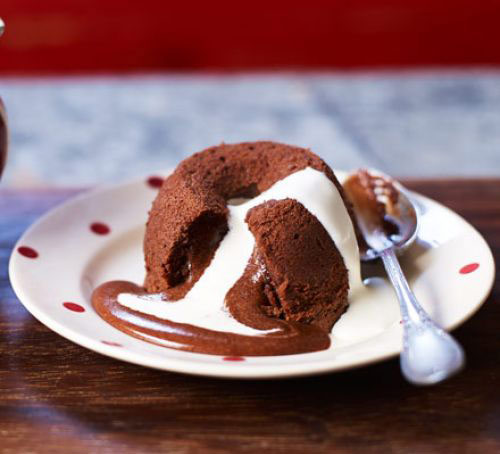
\includegraphics[width=0.7\textwidth]{Fotos/foto_sweet} \end{center}
\clearpage
\receitaemoji{Creme Brulé}{
\begin{itemize}
	\item 320g de creme de leite fresco
	\item Essência de baunilha
	\item 4 gemas
	\item 60g de açúcar fino
\end{itemize}
}{
\begin{enumerate}
	\item Esquentar o creme de leite junto com a baunilha
	\item Bater as gemas separadamente e acrescentar o açúcar
	\item Verter o creme quente sobre as gemas e ao mesmo tempo ir batendo
	      constantemente (temperagem) com um fouet. Evitar formar espuma
	      \begin{itemize}
		      \item É muito importante ir batendo, senão coagula e se perde a cremosidade.
	      \end{itemize}
	\item Verter os ramequins até preencher 2/3.
	\item Aquecer o forno a 150/180 $^\circ$C
	\item Colocar os ramequins numa forma e acrescentar água quente até no máximo
	      metade da altura dos ramequins.
	      \begin{itemize}
		      \item É basicamente um cozimento a banho maria no forno.
		      \item Se não tiver ramequins que suportam altas temperaturas, talvez dê para
		            utilizar xícaras ou potinhos de vidro.
	      \end{itemize}
	\item Levar ao forno por 30 a 40 minutos. Remover
	\item Esfriar na bancada. Depois, levar à geladeira sem cobrir, para não
	      formar uma película.
	\item Antes de servir, espalhar açúcar na superfície e passar o maçarico para
	      caramelizar.
\end{enumerate}
}

\receitatrescols{Overnight Oats}{

	\textsc{receita 1}\checkmark
	\begin{itemize}
		\item morango amassado
		\item açúcar ou maple ou mel
		\item 0,5 xícara de aveia
		\item 0,5 xícara de iogurte (grego)
		\item 0,5 limão espremido
		\item 0,5 xícara de leite
		\item Cobertura: morangos e framboesas
	\end{itemize}

	\textsc{receita 2}
	\begin{itemize}
		\item raspas de meia laranja
		\item açúcar ou maple ou mel
		\item amora preta amassada
		\item 15g de gengibre cristalizado
		\item 1 frasco de iogurte
		\item Cobertura: Amora preta
	\end{itemize}

	\textsc{receita 3}
	\begin{itemize}
		\item 10 g de chocolate em pó
		\item 20 g de aveia
		\item canela
		\item açúcar ou maple
		\item essência de baunilha
		\item 15 g de manteiga de amendoim
		\item 1 frasco de iogurte
		\item Cobertura: raspas de chocolate, framboesa e manteiga de amendoim
	\end{itemize}

}{

	\textsc{receita 4}
	\begin{itemize}
		\item 50 g de manga amassada
		\item 1 colher sopa de coco ralado
		\item 20 g de aveia
		\item essência de baunilha
		\item açúcar ou maple
		\item 1 frasco de iogurte
		\item Cobertura: manga em cubinhos e coco ralado
	\end{itemize}

	\textsc{receita 5}
	\begin{itemize}
		\item 1 cenoura ralada
		\item 20 g de aveia
		\item canela, noz moscada, baunilha
		\item maple ou açúcar
		\item 1 frasco de iogurte
		\item Cobertura: banana e nozes
	\end{itemize}

	\textsc{receita 6}
	\begin{itemize}
		\item 40 g de abacaxi picado
		\item 1 colher de sopa de coco ralado
		\item essência de baunilha
		\item 1 frasco de iogurte
		\item 1 colher de sopa de mel
		\item 20 g de aveia
	\end{itemize}
}{

	\textsc{receita 7}
	\begin{itemize}
		\item 10 g de chocolate em pó
		\item 1 colher de sopa de manteiga de amêndoas
		\item pitada de sal
		\item 1 frasco de iogurte
		\item 1 colher de sopa de mel
		\item 1 colher de sopa de coco ralado
		\item 20 g de aveia
	\end{itemize}

	\textsc{receita 8}
	\begin{itemize}
		\item 1 pote de iogurte
		\item Meia xícara de aveia
		\item Mel, aprox 20mL
		\item Chocolate meio amargo ralado
		\item Fruta congelada
	\end{itemize}

} {
	\begin{enumerate}
		\item Misturar tudo e guardar na geladeira no dia anterior.
		\item No dia seguinte colocar a cobertura.
	\end{enumerate} }


\receitaemoji{Crepe\label{rec:crepe}}{
		\begin{itemize}
			\item 1 ovo
			\item 2 colheres de chá de açúcar
			\item 1 pitada de sal
			\item 250 mL de leite integral
			\item 100g de farinha de trigo
			\item 20g de manteiga mole, derretida
			\item essência de baunilha, licor de laranja ou qualquer aromatizante de
			      preferência
		\end{itemize}
	}{
		\begin{enumerate}
			\item Juntar o ovo, açúcar, sal e bater com fouet. Mixer elétrico pode
			      desvirtuar a massa.
			\item Acrescentar 100mL de leite e misturar.
			\item Acrescentar a farinha de mexer bem até desfazer os grumos.
			\item Acrescentar aos poucos o restante do leite de misturar bem.
			\item Acrescentar a manteiga e misturar.
			\item Acrescentar o aromatizante.
			\item Deixar a massa repousar por pelo menos 1h antes de fritar. Ideal é
			      preparar com 5 horas de antecedência.
			\item Untar bem uma frigideira e aquecer em fogo médio/alto. Colocar uma
			      quantidade que preencha a frigideira bem finamente. Geralmente não precisa
			      untar a frigideira novamente.
			\item Colocar alguma cobertura se desejar. No caso do molho Suzette (receita
			      \ref{rec:molho_suzette}), se dobra o crepe em 4 e depois mergulha no molho,
			      ambos quentes, e é servido imediatamente.
		\end{enumerate}
	}

\receitaemoji{Molho Suzette para Crepe\label{rec:molho_suzette}}{
		\begin{itemize}
			\item 150 mL de suco de laranja
			\item 60 g de manteiga sem sal
			\item 40 g de açúcar
			\item 1 colher de sopa de licor de laranja
			\item raspas de laranja
		\end{itemize}
	}{
		\begin{enumerate}
			\item Derreter a manteiga em fogo médio e acrescentar o açúcar até
			      caramelizar.
			\item Acrescentar o suco de laranja, o licor e as raspas.
		\end{enumerate}
	}

\receitaemoji{Panqueca doce}{

		\textsc{30 panquecas}

		\begin{itemize}
			\item 3 ovos
			\item Meio litro de leite integral
			\item 40g de manteiga sem sal
			\item 40g de açúcar branco
			\item 2g de sal
			\item 225g de farinha de trigo
			\item rum, licor ou essência de baunilha ou aromatizante.
		\end{itemize}

		\textsc{10 panquecas}
		\begin{itemize}
			\item 1 ovo
			\item 0,3 xícara de leite
			\item 0,3 de xícara de creme de leite
			\item 1 colher de sopa de açúcar
			\item 0,75 xícara de farinha de trigo
			\item 1 pitada de sal
			\item 1 colher de sopa de manteiga derretida
			\item 0,5 colher de chá de essência de baunilha ou aromatizante.
		\end{itemize}
	}{
		\begin{enumerate}
			\item Peneirar a farinha junto com o sal e o açúcar
			\item Fazer um espaço no meio da farinha, acrescentar os ovos e ir misturando
			      com um fouet. Um misturador elétrico pode desvirtuar.
			\item Colocar o leite aos poucos para não formar pelotas, enquanto mistura
			\item Em panela separada, derreter a manteiga e juntar à massa, misturar.
			\item Acrescentar o aromatizante.
			\item Descansar a massa na geladeira por no mínimo 1h, idealmente 5.
			\item Untar uma frigideira e levar ao fogo médio/alto.
			\item Colocar uma quantidade de massa suficiente para cobrir o fundo da
			      frigideira, bem fino.
			\item Virar com uma espátula quando as bordas começarem a se soltar.
		\end{enumerate}
	}

\receitaemoji{Bolo de chocolate}{ % todo: adequar o texto.
		\textsc{Bolo de chocolate}
		\begin{itemize}
			\item 4 ovos
			\item 1 xícara (chá) de açúcar
			\item 1 xícara (chá) de chocolate em pó
			\item 1 xícara (chá) de óleo
			\item 1 xícara (chá) de água
			\item 2 xícaras (chá) de farinha de trigo
			\item 1 colher (sopa) de fermento
			\item Manteiga, farinha e chocolate para untar e polvilhar
		\end{itemize}
		\textsc{Calda de ganache}
		\begin{itemize}
			\item 200g de chocolate meio amargo
			\item 3/4 de xícara (chá) de creme de leite fresco
		\end{itemize}
	}{
		\begin{enumerate}
			\item Preaqueça o forno a 180ºC (temperatura média). Unte uma forma redonda ou
			      de pudim com manteiga, formando uma camada fina e uniforme.
			\item Faça uma misturinha meio a meio de chocolate em pó e farinha, e polvilhe
			      a forma toda. Desta maneira, o bolo não fica com aquela casquinha branca de
			      farinha. Reserve. Numa tigela, coloque a farinha, passando pela peneira.
			\item Na batedeira, ou numa tigela, coloque o açúcar e o chocolate em pó,
			      passando por uma peneira. Junte os ovos e o óleo. Na velocidade baixa (para
			      o chocolate não subir), bata os ingredientes, até que estejam bem
			      misturados.
			\item Aumente a velocidade e bata por mais alguns minutos. Caso prefira fazer
			      à mão, use um batedor de arame. Se estiver usando a batedeira, abaixe a
			      velocidade novamente e, aos poucos, vá adicionando a água e a farinha,
			      alternadamente, batendo apenas para misturar.
			\item Por último, adicione o fermento. Transfira a massa para a forma
			      preparada e leve ao forno preaquecido para assar por 30 minutos, até que o
			      palito saia limpo ao ser espetado no bolo.
			\item Retire do forno e deixe esfriar por 15 minutos. Coloque um prato de bolo
			      sobre a forma e, com o auxílio de um pano de prato vire de uma vez. Somente
			      quando o bolo estiver frio, espalhe a calda. Sirva a seguir.
		\end{enumerate}
	}

\receitaemoji{Mousse de chocolate}{
		\begin{itemize}
			\item 100 g de chocolate Cicao Mix (mistura de ao leite e meio-amargo)
			      \footnote{Essa quantia de chocolate foi dobrada. É possível que não precise
				      dobrar a quantidade caso use um chocolate mais duro.}
			\item 35 g de água
			\item Gelo
		\end{itemize}
	}{
		\begin{enumerate}
			\item Cortar o chocolate em pedaços grandes
			\item Misturar a água
			\item Levar ao microondas por 20 segundos.
			\item Mexer bem, levar por mais 20 segundos.
			\item Mexer, garantir que a mistura está bastante leve, sem grumos de
			      chocolate.
			\item Fazer um banho de gelo.
			\item  Colocar o chocolate no banho e bater bastante
			      com um mixer até ficar com uma consistência firme.
			\item Transferiro para um potinho
			\item Levar à geladeira por 1h para tomar consistência. Comer com moderação
		\end{enumerate}
	}

\receitaemoji{Mingau de aveia}{
		\begin{itemize}
			\item 200 mL de leite (ou 3/4 xícara de leite)
			\item 20 g de aveia   (ou 1/3 xícara de aveia)
			\item 1 punhado de cranberries
			\item (opcional) açúcar ou mel
			\item (opcional) gotas de chocolate
			\item (optional) amêndoas picadas para guarnecer
		\end{itemize}
	}{
		\begin{enumerate}
			\item Misturar tudo, colocar no fogo médio, mexendo sempre, até ficar espesso
			\item Colocar o guarnecimento, se desejar.
		\end{enumerate}
	}

\receitaemoji{Torta de Iogurte}{
	\begin{itemize}
		\item 4 ovos separados
		\item 70 g de açúcar
		\item 350 g de iogurte grego
		\item 40 g de maizena
		\item 4 g de fermento royal
		\item raspas de limão
		\item baunilha
	\end{itemize}
}{
	\begin{enumerate}
		\item Bater as claras em neve e reservar
		\item Bater as gemas com o açúcar até ficar bem claro e aumentar o volume.
		\item Acrescentar o iogurte, as raspas e a baunilha às gemas batidas e
		      misturar bem
		\item Acrescentar a maizena junto com o fermento à mistura anterior até
		      incorporar bem.
		\item Acrescentar as claras em neve aos poucos, com auxílio de uma espátula.
		      Não usar batedeira. Usar movimentos largos, para não remover o ar.
		\item Colocar em uma forma de 22 cm de diâmetro.
		\item Assar por 40-45 minutos a 170\grau{} C.
	\end{enumerate}
}

\receitaemoji{Bolo de cenoura}{
	\begin{itemize}
		\item 3 cenouras grandes cortadas em rodelas
		\item 1 xícara de açúcar
		\item 0.5 xícara de óleo
		\item 3 ou 4 ovos
		\item 2 xícaras de farinha de trigo
		\item 1 colher de sopa de fermento
		\item 0.5 colher de chá de sal
		\item Manteiga para untar
	\end{itemize}
}{
	\begin{enumerate}
		\item Colocar as cenouras, açúcar, óleo e ovos no liquidificador, bater e
		      reservar
		\item Colocar a farinha de trigo, fermento, sal numa cuia, misturar bem,
		      adicionar os líquidos da etapa anterior, homogeneizar mas não bater muito.
		\item Untar a forma, colocar em forno pré-aquecido a 200\grau{} C por 40
		      minutos.
	\end{enumerate}
	\fotoreceita{0.7\textwidth}{./Fotos/bolo_cenoura.jpg}
}

\receitaemoji{Pão de mel em cubos}{
	\begin{itemize}
		\item 250 g de mel
		\item 200 g de açúcar
		\item 450 g de farinha de trigo
		\item 200 g de farinha  de amêndoas
		\item 100 g de nozes picadas
		\item 100 g de avelãs picadas
		\item 1/2 colher de chá de cardamomo moído
		\item 1/2 colher de chá de cravo em pó
		\item 1 colher de chá de canela em pó
		\item 100 g de frutas cristalizadas (p.e. cascas de laranja, de limão)
		\item 15 g de carbonato de amônio
		\item 4 colheres de sopa de rum1 ovo
		\item Manteiga e farinha para a assadeira
		\item Película de plástico para abrir a massa
		\item 3 colheres de sopa de geléia de damasco ou similar, 1 colher de sopa
		      de rum, 200 g de chocolate meio amargo para cobertura.
		\item 20 g de pistache picado, 50 g de cereja em calda, 50 g de amêndoas sem
		      pele, 50 g de nozes.
	\end{itemize}
}{
	\begin{enumerate}
		\item Numa panela levar o mel e açúcar em fogo baixo, misturando sempre, até
		      o açúcar se dissolver. Passar a massa para uma tigela e deixar esfriar.
		\item Pré-aquecer o forno a 175 \grau C.
		\item Untar uma assadeira com manteiga e passar um pouco de farinha
		\item Misturar a farinha e as amêndoas, avelãs, nozes, temperos e frutas
		      cristalizadas.
		\item Dissolver o carbonato de amônio com rum
		\item Adicionar um ovo à mistura de mel com açúcar e ir colocando aos poucos
		      a mistura de carbonato de amônio
		\item Amassar bem a massa e abri-la de modo uniforme entre as duas lâminas
		      de filme de plástico, na espessura da assadeira.
		\item Tirar a película de plástico e colocar a massa na assadeira. Assar por
		      20 minutos na grade do meio.\footnote{Feito para o nosso casamento!}
	\end{enumerate}
}



%%% Local Variables:
%%% mode: latex
%%% TeX-master: "main"
%%% End:


% \begin{itemize} \item \end{itemize}

\end{document}
